\documentclass[a4paper, 12pt, titlepage]{article}

\usepackage[utf8]{inputenc}
\usepackage{geometry}
\usepackage{polski}
\usepackage{graphicx}
\usepackage{float}
\usepackage{etoolbox,refcount}
\usepackage{multicol}
\usepackage{fancyhdr}
\usepackage{listings}
\usepackage{amsmath}
\usepackage{tabularx}
\usepackage{svg}

\newgeometry{left=2.5cm, right=2.5cm, bottom=2.5cm, top=2.5cm}

\lstset{
    basicstyle=\footnotesize
    language=Matlab,
    basicstyle=\ttfamily,
    keepspaces=true,
    frame=single,
    tabsize=4,
    showspaces=false,
    showstringspaces=false,
    backgroundcolor = \color{lightgray}
}

\author{Konrad Czaja, Adrian Jałoszewski,\\Dorota Kowalik}
\title{Akwizycja danych z sensorów urządzeń mobilnych}
\date{11 października 2017}
    
\begin{document}
    \maketitle
	\section{Cel ćwiczenia}
        Celem ćwiczenia jest implementacja algorytmu zliczającego 
        kroki na podstawie danych zebranych z czujników urządzenia
        mobilnego z systemem Android. Algorytm ten powinien być
        odporny na zachowania inne niż chód oraz możliwy do 
        zastosowania w ciągłej akwizycji danych.
    \section{Wykonanie ćwiczenia}
        \subsection{Umieszczenie telefonu}
            Telefon został umieszczony przy szyi tak aby w trakcie
            obrotów w jak najmniejszym stopniu podlegał sile
            odśrodkowej w przypadku obrotów.
        \subsection{Algorytm przetwarzania danych}
            Przedstawiony algorytm ma zastosowanie dla przypadku kiedy
            dane z całego przebiegu są już dostępne do analizy.
            \begin{figure}[H]
                \centering
                \includegraphics[width=0.5\columnwidth]{algorytm.png}
                \caption{Schemat blokowy algorytmu}
            \end{figure}\noindent
            \subsubsection{Połączenie z telefonem}
                Połączenie z telefonem zostało nawiązane przez
                aplikację mobilną pozwalającą na akwizycję danych
                z urządzenia. Należało ustawić flagę uruchamiającą
                akcelerometr oraz włączającą logowanie danych.
                Częstotliwość próbkowania została ustawiona na wysoką --
                jest to wartość określona w dokumentacji jako 100Hz. 
                Po czasie przeznaczonym na zbieranie danych (w tym
                przypadku 15s) flaga logowania próbek jest zerowana, 
                a dane są pobierane jako lista składowych przyśpieszenia
                oraz wektor czasu.
                \lstinputlisting{./scripts/data_aq.m}
            \subsubsection{Wyznaczenie wartości przyśpieszenia}
                Dane są umieszczane jako trzy wykresy, z oznaczeniem
                poszczególnych składowych. Następnie liczona jest
                wartość przyśpieszenia dla każdej próbki.
                \lstinputlisting{./scripts/data_capture.m}
            \subsubsection{Wstępna filtracja danych}
                Pierwszym krokiem w filtracji jest usunięcie składowej
                stałej. Otrzymany w ten sposób sygnał jest wycentrowany
                względem zera oraz została od niego odjęta grawitacja.
                Jako maksymalną częstotliwość chodu zostało przyjęte 3 
                Hz. Jest to przypadek biegu. Wszystkie częstotliwości
                powyżej są traktowane jako zakłócenia.
                \newpage
                \lstinputlisting{./scripts/simple_filtering.m}
                Współczynnik filtru $b$ został zaimportowany z edytora
                filtrów:
                \begin{figure}[H]
                    \centering
                    \includegraphics[width=0.9\columnwidth]{filtr.png}
                    \caption{Ustawienia filtru}
                \end{figure}\noindent
            \subsubsection{Usunięcie gwałtownych ruchów}
                Z zebranych danych wynika, że wszystkie skoki jakie 
                zostały zmierzone mają amplitudę powyżej $6 \frac{
                    \mathrm{m}}{\mathrm{s}}$ dlatego też takie wartości
                zostały usunięte z sygnału. Zostało to dokonane przez
                wyzerowanie wszystkich wartości dodatnich wokół pomiarów
                przekraczających próg.
                \lstinputlisting{./scripts/peak_deletion.m}
            \subsubsection{Zliczanie kroków}
                Zliczanie kroków zostało zrealizowane poprzez zliczenie
                szczytów w sygnale powstałym przez odfiltrowanie.
                Wartości ujemne zostały usunięte, gdyż nie są istotne
                dla dalszych rozważań. Do zliczenia szczytów została 
                wykorzystana funkcja \texttt{findpeaks} z odchyleniem
                standardowym sygnału wynikowego jako minimalna wysokość
                szczytu.
                \lstinputlisting{./scripts/steps_detection.m}
            \subsubsection{Wyrysowanie wyników}
                \lstinputlisting{./scripts/plotting.m}
    \section{Pomiary oraz ich analiza}
        Dane zebrane z czujników przed przetworzeniem są przebiegami
        składowych przyśpieszenia zarejestrowanego przez akcelerometry.
        Zależnie od położenia przebiegi te posiadają składową stałą.
        \begin{figure}[H]
            \centering
            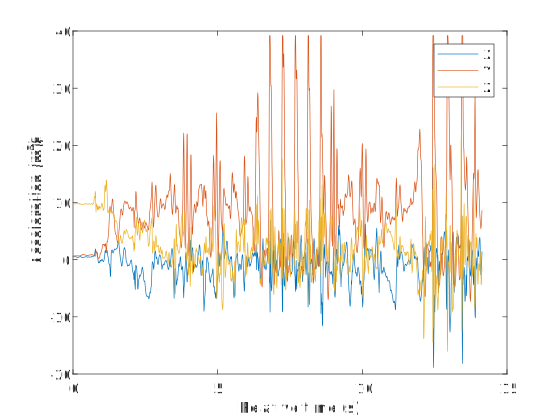
\includegraphics[width=0.49\columnwidth]
                {krok_dziala1g.png}
            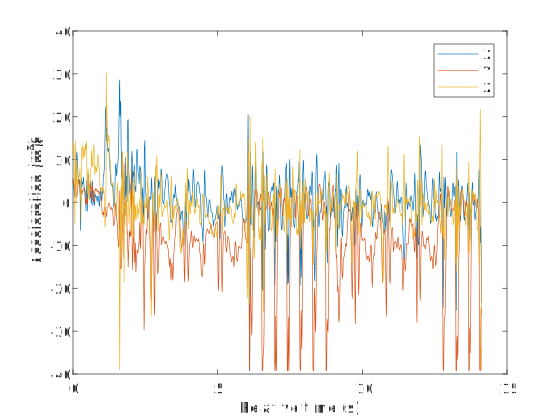
\includegraphics[width=0.49\columnwidth]
                {krok_dziala2b.png}
            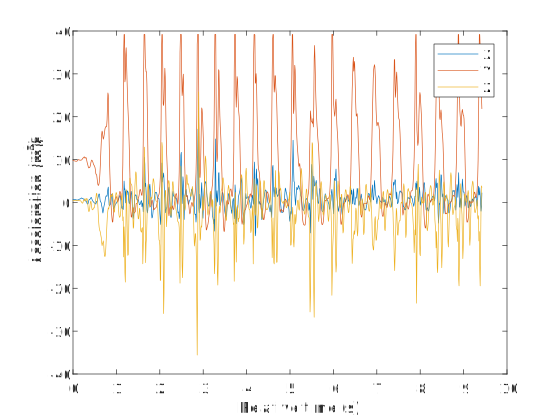
\includegraphics[width=0.49\columnwidth]
                {skok1_a.png}
            \caption{Dane zebrane z czujników}
        \end{figure}\noindent
        Dla przypadku zawierającego tylko podskoki wartość
        przyśpieszenia kształtowała się następująco:
        \begin{figure}[H]
            \centering
            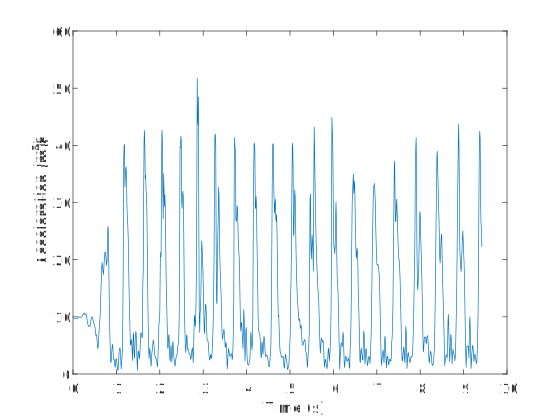
\includegraphics[width=0.8\columnwidth]
                {skok1.png}
            \caption{Wartość przyśpieszenia przy samych podskokach}
        \end{figure}\noindent
        Po zastosowaniu algorytmu dla przebiegu z pominięciem kroku
        usuwającego podskoki sygnał kształtuje się następująco:
        \begin{figure}[H]
            \centering
            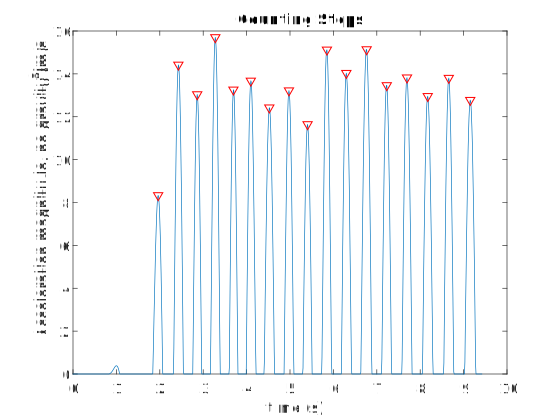
\includegraphics[width=0.8\columnwidth]
                {skok1_2.png}
            \caption{Zliczone i zaznaczone rozpoznane podskoki}
        \end{figure}\noindent
        W przypadku, gdzie występowały zarówno podskoki jak i zwykły
        chód przebieg po zastosowaniu algorytmu bez usuwania podskoków
        kształtuje się następująco:
        \begin{figure}[H]
            \centering
            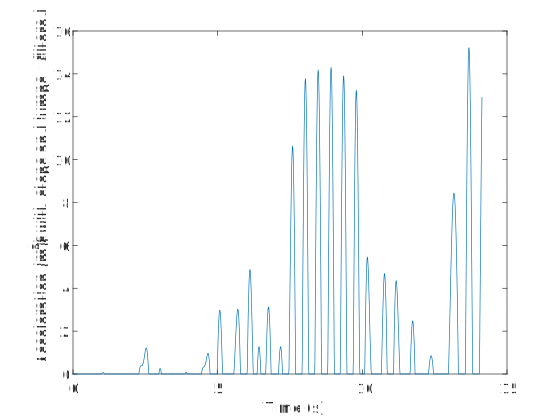
\includegraphics[width=0.8\columnwidth]
                {krok_dziala1a.png}
            \caption{Kroki i podskoki}
        \end{figure}\noindent
        Na podstawie pomiarów nasunął się wniosek przyjęcia
        rozgraniczenia kroków i podskoków progiem $6 \frac{
            \mathrm{m}}{\mathrm{s}}$. Podobne rezultaty były uzyskiwane
        dla innych przemarszy z podskokami.
        \newpage
    \section{Wyniki}
        Rozwiązanie zostało przetestowane dla dwóch przemarszy
        z podskokami różniącymi się tym czy najpierw następuje marsz
        czy podskoki.
        \subsection{marsz -- podskoki -- marsz -- podskoki}
            \begin{figure}[H]
                \centering
                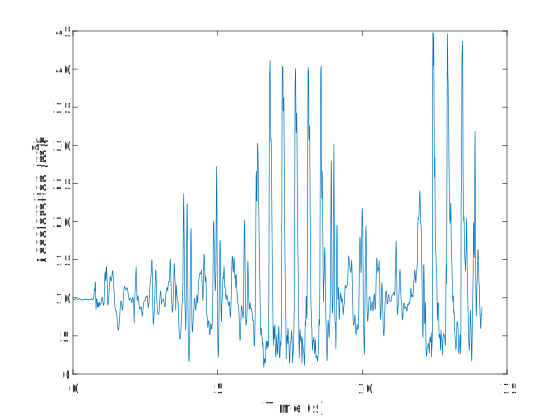
\includegraphics[width=0.7\columnwidth]
                    {krok_dziala1f.png}
                \caption{Przed filtrowaniem}
            \end{figure}\noindent
            \begin{figure}[H]
                \centering
                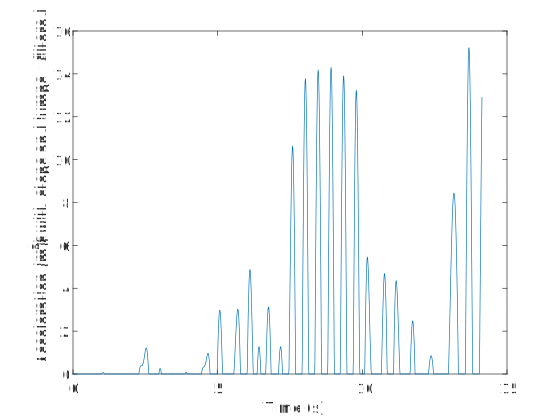
\includegraphics[width=0.7\columnwidth]
                    {krok_dziala1a.png}
                \caption{Bez wycięcia podskoków}
            \end{figure}\noindent
            \begin{figure}[H]
                \centering
                \includegraphics[width=0.7\columnwidth]
                    {krok_dziala1b.png}
                \caption{Po wycięciu podskoków}
            \end{figure}\noindent
        \subsection{podskoki -- marsz -- podskoki -- marsz}
            \begin{figure}[H]
                \centering
                \includegraphics[width=0.7\columnwidth]
                    {krok3a.png}
                \caption{Przed filtrowaniem}
            \end{figure}\noindent
            \begin{figure}[H]
                \centering
                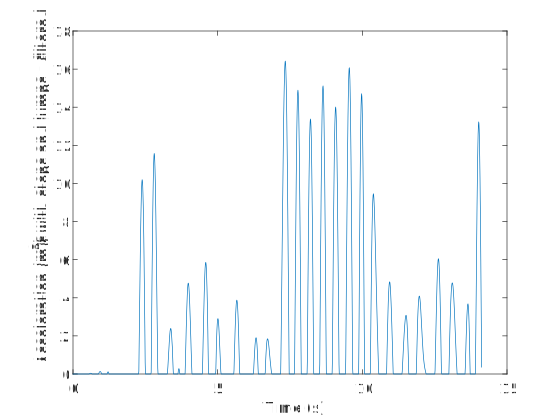
\includegraphics[width=0.7\columnwidth]
                    {krok3.png}
                \caption{Bez wycięcia podskoków}
            \end{figure}\noindent
            \begin{figure}[H]
                \centering
                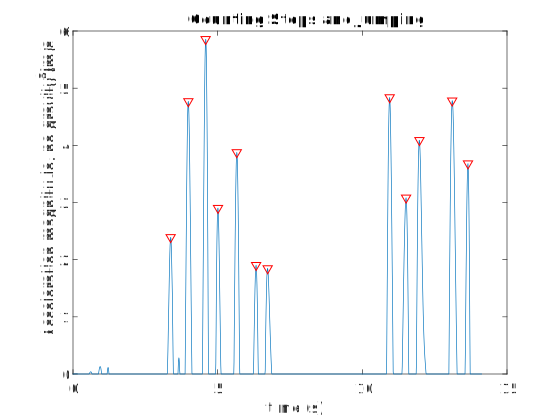
\includegraphics[width=0.7\columnwidth]
                    {krok3b.png}
                \caption{Po wycięciu podskoków}
            \end{figure}\noindent
    \section{Podsumowanie i obserwacje}
        Nie udało nam się zaimplementować ciągłego wczytywania danych
        oraz ich obróbki. Wynikło to z tego, że za dużo czasu zostało
        poświęcone na sensowną metodę usunięcia podskoków.
        \\ \\
        Ze względu na naturę zastosowanego przez nas filtru początkowe
        pomiay zostały usunięte. Dlatego też był potrzebny pewien
        czas rozbiegu dla programu po którym dopiero zaczynały napływać
        wyniki możliwe do dalszej obróbki.
        \\ \\
        Po rozbiegu program poprawnie liczy kroki, skutecznie pomijając
        podskoki. Zostało to zweryfikowane poprzez zliczanie kroków i
        porównanie uzyskanej liczby z uzyskanym w programie wynikiem.
        \\ \\
        Zaproponowany algorytm nie bierze pod uwagę przypadku gdy mamy
        do czynienia z nietypowym, skocznym chodem. W tym przypadku
        część kroków może być sklasyfikowanych jako podskoki i są
        usuwane.
\end{document}
